
% POSTER EXAMPLE
%
% This is an example of a relatively sane poster. The box structure (and the
% narrative in general) is what I would expect, but it is completely
% non-mandatory; you may include whatever you want. Preferably, erase the
% existing box structure after you read it, and start from scratch.
%
% The main communication requirements for the poster that should be satisfied
% are as such:
%
% - At the defense, it should help you talk for around 10 minutes about your
%   thesis, and convince the committee that you did something interesting and
%   sufficiently complicated. Prepare pictures that explain your main results.
%
% - It should quickly communicate the main idea of your thesis to a random
%   educated by-walker. Ideally, a moderately-witted MFF graduate who has never
%   heard about your thesis before should be able to get the main "rough idea"
%   in less than 1 minute by just looking at the poster.

% modify the fontscale parameter to make everything slighly bigger or smaller.
\documentclass[portrait,a0paper,fontscale=0.25]{baposter}

\usepackage[utf8]{inputenc}
\usepackage[T1]{fontenc}

% FONT CHOICES
% Posters do not need to be PDF/A; you can choose any relatable font from the
% TeX font catalogue without much risk. Sans-serif fonts are suggested for the
% posters; see https://tug.org/FontCatalogue/sansseriffonts.html
\usepackage[sfdefault]{Fira Sans}
%\usepackage[default]{droidsans}
%\usepackage[math]{iwona}
%\usepackage[defaultfam]{montserrat}
%\usepackage{cmbright}
%\usepackage{yfonts}\renewcommand{\familydefault}{\frakdefault}

\usepackage{color}
\usepackage{graphicx}
\usepackage{amssymb,amsmath}
\usepackage[export]{adjustbox} %allows using valign with \includegraphics

\renewcommand{\arraystretch}{1.5}

\usetikzlibrary{positioning}

% A WORD ABOUT COLORS
%
% This template is prepared with a relatively neutral gray background that
% gives decent box borders (with white and darker gray), does not clash with
% many colors (except for violet-brown and other mushroomish colors, perhaps)
% and gives a lot of space for highlighting stuff.
%
% Generally, other color variations are good too; there are no strict rules on
% the colors. Good choices include:
%
% - white backgrounds and differentiation of box headers by color (see
%   headerFontColor)
%
% - various slightly tinted backgrounds (try red!10 instead of black!3)
% 
% - dark backgrounds
%
% Keep in mind:
% - The normal "informative" text and figures should be DARK on LIGHT
%   background, not the other way around.
%
% - If you want a dark background, soften (darken) the box backgrounds a bit so
%   that they do not "shine" too much from the poster. Use \color{white} for
%   the heading, and switch the UK/MFF logos to white (see contents of logos/).
%
% - Do not mix too many color hues together. Most hues have their widely
%   accepted meaning (green: good result, red: problem, blue: information,
%   yellow: highlighter, brown: serious problem, violet: something really
%   weird/interesting/magic, depending on the shade).

\begin{document}

\color{black!80} % default font color
\begin{poster}{grid=false,
	eyecatcher=true,
	background=plain,
	bgColorOne=black!3, % background color
	columns=2,
	headerborder=none,
	textborder=none,
	headershape=rectangle,
	headershade=plain,
	boxshade=plain,
	boxColorOne=white,
	headershade=plain,
	headerColorOne=black!15, % box header background color
	headerFontColor=black,
	}%
	{
\includegraphics[height=7em]{logos/mff-black.pdf}}
    {Evoluce robotů v simulovaném\vspace*{4px} fyzikálním prostředí}
	{\vspace{1ex} Marek Bečvář}
	{
\includegraphics[height=7em]{logos/uk-red.pdf}}


%
% LEFT COLUMN
%

\begin{posterbox}[column=0,name=uvod]{Úvod}
Pro řešení různorodých problémů se nám může hodit využívat metod evolučních
algoritmů. Jedná se o přírodou inspirované optimalizační algoritmy, které
napodobováním přírodních procesů hledají nejlepší řešení pro zadané cíle.

Práce s těmito algoritmy ale může být velmi složitá kvůli velkému množství
parametrů a nastavení, se kterými je potřeba najednou při experimentech
pracovat.

% \begin{center}\begin{tikzpicture}[ultra thick, inner sep=1ex]
% \node[rectangle, rounded corners=1ex, draw=red!80!black, color=red!80!black, font=\huge\bfseries, rotate=21] {Problem!};
% \end{tikzpicture}\end{center}
\end{posterbox}

\begin{posterbox}[column=0, name=goals, below=uvod, headerColorOne=cyan!60, boxColorOne=cyan!20]{Cíle práce}
% \textbf{Hlavním cílem} práce bylo vytvořit platformu, která umožní provádět
% experimenty s evolučními algoritmy, dostupnou pro uživatele různých úrovní
% specializace. Evoluční algoritmy jsou v práci využívány pro vývoj robotů v
% simulovaném prostředí.
\textbf{Hlavní cíl:} platforma pro experimenty s evolučními algoritmy, dostupná
pro uživatele různých úrovní specializace. Evoluční algoritmy v projektu
vyvíjí roboty v simulovaném prostředí.
\\\\
% \textbf{Vedlejším cílem} práce bylo pomocí experimentů ověřit základní hypotézu,
% že pro vývoj složitějších robotů (více stupňů volnosti) potřebujeme složitější
% evoluční algoritmy.
\textbf{Vedlejší cíl:} experimentálně ověřit hypotézu, že pro
vývoj složitějších robotů (více stupňů volnosti) potřebujeme složitější
evoluční algoritmy.
\end{posterbox}

\begin{posterbox}[column=0, name=something1, below=goals]{Využité technologie}
Celý projekt je pro přehlednost a rozšiřitelnost napsaný v~programovacím jazyce
Python.
\\\\
Pro lepší čitelnost a rozšířitelnost naší platformy jsme se rozhodli nevyužít
již existující knihovny pracující s evolučními algoritmy. Místo toho jsme
vytvořili vlastní implementace nejpoužívanějších základních bloků, ze kterých
mohou být evoluční algoritmy poskládány.
\\\\
Simulované fyzikální prostředí je důležitou částí tohoto projektu. S ohledem na
naše požadavky jsme pro tento účel zvolili fyzikální prostředí \emph{MuJoCo}
zpřístupněné pomocí knihovny \emph{Gymnasium} (dříve \emph{OpenAI Gym}).
\\\\
Platforma umožňuje využít grafické rozhraní pro podrobnou konfiguraci
experimentů, které bylo implementována pomocí knihovny \emph{PySimpleGUI}.

\begin{center}
    \vspace{10px}
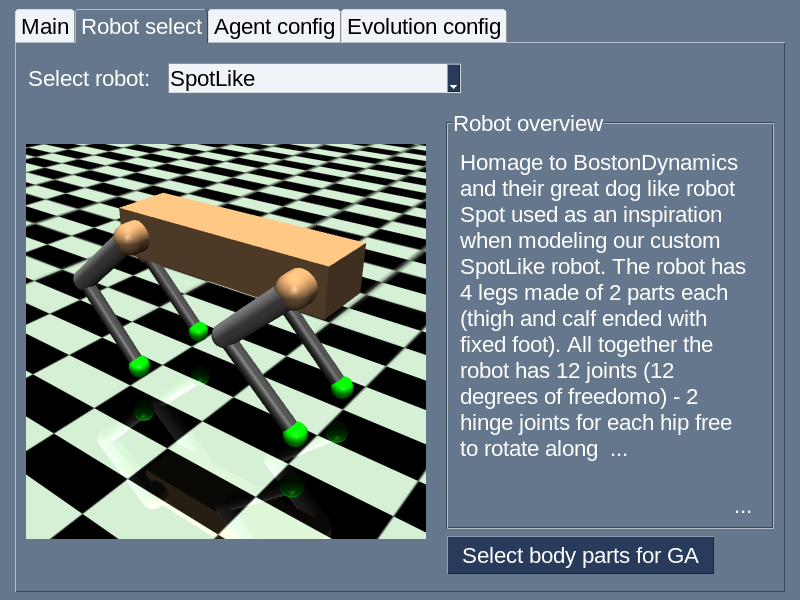
\includegraphics[width=0.95\linewidth]{../../BP/img/GUI_robot_tab_spot.jpg}
\end{center}
\end{posterbox}

% \begin{posterbox}[column=0, name=something2, below=something1, headerColorOne=yellow!80!orange!95!black, boxColorOne=yellow!33]{Golden rule of posters}
% For each $p \in P$ where $P$ is a set of posters:
% $$ \textsc{Success}(p) = \frac{\textsc{Clarity}(p)}{\textsc{TimeToViewerAttention}(p)} $$
% \end{posterbox}

%
% FOOTER
%

\begin{posterbox}[column=0, span=2, name=footer, below=something1,
	textborder=none, headerborder=none, boxheaderheight=0pt,
	boxColorOne=black!3]{}
\small
Děkuji tímto panu RNDr. Františku Mrázovi, CSc. za vedení a rady při
vypracování této práce.
\end{posterbox}

%
% RIGHT COLUMN
%
% It is usually best to fill most of the poster with your results and
% conclusions. Again, use simple annotated pictures wherever possible. Plots
% with measurements are perfect, tables are also good.
%

\begin{posterbox}[column=1, name=result1]{Platforma}
\begin{center}
\vspace{5px}
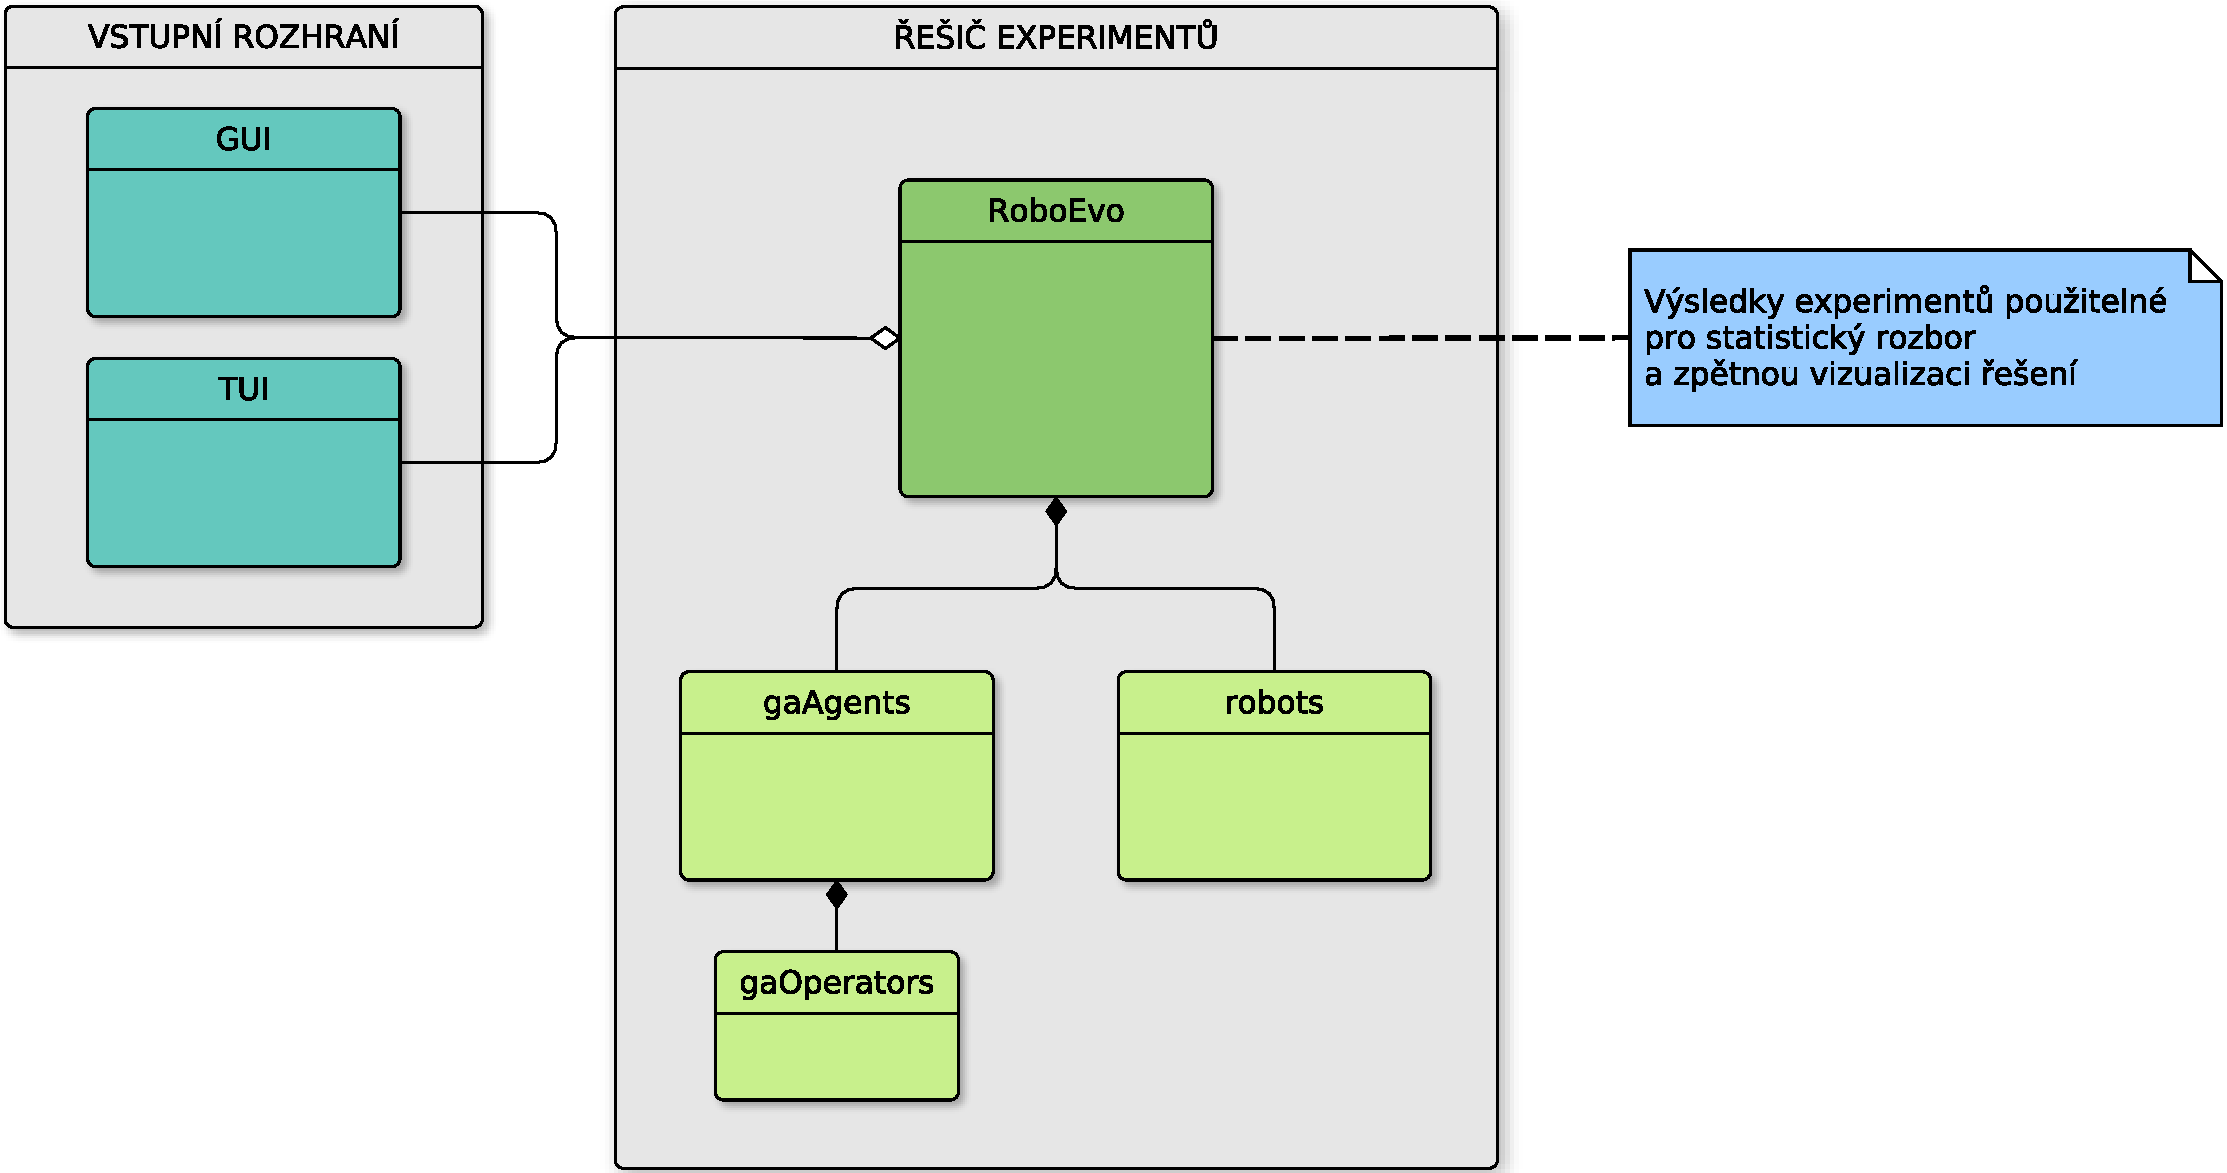
\includegraphics[width=0.9\linewidth]{../../BP/img/BP_imp_graph.pdf}
\end{center}

Prací vznikla platforma pro snadné experimentování s~evolučními algoritmy
umožňující podrobnou, interaktivní konfiguraci experimentů v grafickém
rozhraní, a zároveň spouštění a statistické vyhodnocování většího množství
experimentů v textovém rozhraní. 

Pro maximální efektivitu je běh evolučních algoritmů paralelizován, využívající
moderních CPU.

Přehledná implementace a dokumentace modulů umožňuje uživateli projekt
jednoduše rozšiřovat (nové typy evolučních algoritmů, nové příklady robotů).

\end{posterbox}

\begin{posterbox}[column=1, name=result2, below=result1]{Ověření hypotézy}

Pro splnění druhého cíle práce jsme zvolili dva typy evolučních algoritmů.
Algoritmy se liší hlavně ve způsobu, jak transformují informace z prostředí na
nastavení motorů robota. 

Jednodušší algoritmus pro nastavení každého z motorů využíval sinusoidu s
vlastními parametry pro každý motor. Složitější algoritmus využíval zkrácenou
Fourierovu řadu opět s parametry pro každý motor.

Experimenty s oběma algoritmy potvrdily, že u~jednoduchých robotů zvládají oba
najít řešení pro zadaný cíl (urazit rovně co největší vzdálenost). Pro
složitého robota (\emph{SpotLike} z ukázky grafické aplikace) byl pouze
složitější algoritmus schopný najít řešení a tak potvrdil základní hypotézu.

\end{posterbox}

\begin{posterbox}[column=1, name=conclusion, below=result2, bottomaligned=something1]{Závěr}
% \begin{itemize}
% \item explain the value of your result to others
% \item point out any applications
% \item if the program is online/opensource/on github, you may highlight it here
% \end{itemize}

Práce splnila cíle, které pro ní byly zadány. Platforma pro provádění
experimentů je přehledná, funkční a stabilní \linebreak (dostupná na OS Windows a Linux).
Projekt zároveň dává nástroje pro vizualizaci řešení a statistické vyhodnocení
dat z~experimentů.

Platforma také umožnila splnění vedlejšího cíle práce a to ověření základní
hypotézy o rozdílných složitostech ovládání robotů.

\begin{center}
    \hspace{100px}
    
\includegraphics[width=0.3\linewidth]{../../BP/img/QRGitlab.png}

    \vspace{-57px} % vspace
    \hspace{-110px} % hspace
    Celý projekt dostupný v \\ \hspace{-100px}Gitlab repozitáři:
\end{center}
\end{posterbox}


\end{poster}
\end{document}
